\chapter{Implementazione}
\label{implementazione}
In questa sezione è descritta l'implementazione del progetto definito nel capitolo precedente. I principali strumenti utilizzati sono Python come linguaggio di programmazione e le librerie Scikit-learn \cite{sklearn} per attuare machine learning e Keras \cite{keras} per realizzare reti neurali.
Di seguito sono elencati i dettagli implementativi delle singole entità, ed i parametri usati durante la fase sperimentale.

\section{Classificatore Random Forest}
\label{imp:randomforest}
Il classificatore Random Forest è stato implementato tramite l'uso della libreria python Scikit-learn \cite{sklearn}. 
Al fine di avere un ambiente di testing facilmente fruibile, è stata creata una classe $MyClassifier$ in grado di gestire la serie di esperimenti effettuata sul classificatore, al fine di testare i differenti parametri di funzionamento e la composizione delle features del dataset. in figura \ref{fig:uml_randomforest} è mostra

\begin{figure}[!htb]
	\centering
	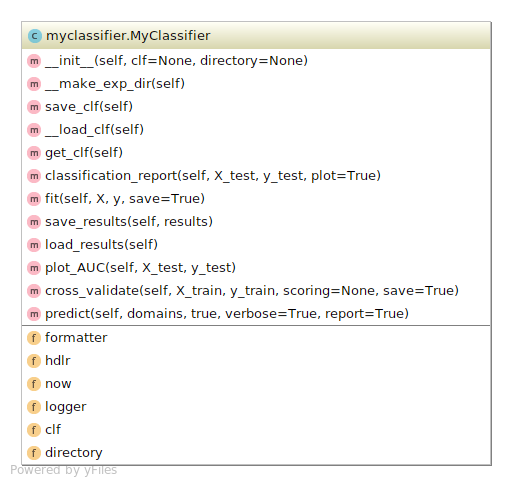
\includegraphics[width=0.7\columnwidth]{figures/uml_randomforest.png}
	\caption{Diagramma UML della classe MyClassifier 			\label{fig:uml_randomforest}}
\end{figure}


\subsection{Dataset}
Il dataset utilizzato per le fasi di training e testing del classificatore è stato definito nella sezione \ref{pro:randomforestdataset}. A livello operativo il dataset è stato generato a partire dai soli nomi di dominio in formato stringa, per i quali sono stati estratti le singole features. Segue una descrizione dettagliata delle features utilizzate per generare il dataset.

\begin{itemize}
\item \textbf{MCRExtractor} si occupa di fornire il rapporto tra caratteri significativi. E' caratterizzato dal parametro che identifica la minima sottostringa da analizzare, composta da 3 caratteri. L'algoritmo cicla per ogni dimensione di n-gramma $\geq 3$ , estrae le tuple di dimensione $i$ dalla stringa e per ogni tupla $s$ presente in una $word$ del dizionario inglese, viene aggiunta la sua lunghezza alla somma dei caratteri significativi della stringa. 
Il risultato è il rapporto tra la somma della lunghezza dei caratteri significativi e la lunghezza totale della stringa.
 
\begin{lstlisting}[language=Python]
min_subtr = 3
maxl = 0
for i in range(min_subtr, len(str(domain_name))):
	tuples = zip(*[str(domain_name)[j::i] for j in range(i)])
	split = [''.join(t) for t in tuples]
	tmpsum = 0
	tmps = []
	for s in split:
		for words in eng_dict:
			if s in words:
				tmpsum += len(s)
				tmps.append(s)

	if tmpsum > maxl:
		maxl = tmpsum
return maxl / int(len(str(domain_name)))
\end{lstlisting}

\item \textbf{NormalityScoreExtractor} estrae il punteggio di normalità degli n-grammi. A differenza del lavoro propsoto in \cite{Schiavoni2014}, si è scelto di estrarre il \textit{normality score} per gli n-grammi di lunghezza 1,2,3,4,5 caratteri, in quanto in fase sperimentale hanno dimostrato di fornire un apporto significativo alla precisione del classificatore. E' definito dal seguente algoritmo, dove il valore $self.n$ identifica la lunghezza dell'n-gramma da valutare. L'algoritmo separa in n-grammi di dimensione $n$ la stringa e per ogni tupla di caratteri $s$, somma il numero di occorrenze di tale tupla all'interno del vocabolario inglese, ritornando il rapporto tra il valore complessivo delle occorenze delle tuple nel vocabolario inglese e la lunghezza della stringa meno $n+1$.

\begin{lstlisting}[language=Python]
if len(str(domain_name)) < self.n:
            return 0
tuples = ngrams(str(domain_name), self.n)
myngrams = (''.join(t) for t in tuples)
scoresum = 0
for s in myngrams:
	counter = 0
    for words in eng_dict:
    	if s in words:
        	counter += 1
    scoresum += counter
return scoresum / (len(str(domain_name)) - self.n + 1)
\end{lstlisting}

\item \textbf{NumCharRatio} estrae il rapporto di caratteri numerici rispetto alla lunghezza della stringa

\begin{lstlisting}[language=Python]
counter = Counter(domain_name)
ncr = 0
for key, value in counter.iteritems():
	if key.isdigit():
		ncr += value

return ncr / len(domain_name)
\end{lstlisting}

\item \textbf{DomainNameLength} estrae la lunghezza del nome di dominio.

\begin{lstlisting}[language=Python]
return (len(domain_name))
\end{lstlisting}

\item \textbf{VowelConsonantRatio} estrae il rapporto tra vocali e consonanti all'interno della stringa.

\begin{lstlisting}[language=Python]
count = 0
vowels = set("aeiou")
for letter in domain_name:
	if letter in vowels:
		count += 1
return count / (len(domain_name) - count)
\end{lstlisting}

\end{itemize}

L'insieme di tali features è stato usato per generare un dataset contenente per ogni nome di dominio le 9 features linguistiche generate a partire dalle stringhe dei nomi di dominio. 

Assieme a tale dataset è stato generato un vettore binario "\textit{target}" da cui il classificatore può verificare la categoria di appartenenza (malevolo o reale) di ogni dominio.

\subsection{Parametri Classificatore}
In particolare i parametri del classificatore utilizzato che sono stati modificati dal loro valore di default sono:
\begin{itemize}
\item \textbf{\texttt{n\_estimators}} = 100. Numero di stimatori da utilizzare nel processo. Il valore è stato deciso come ottimale dopo una serie di test sperimentali preliminari.
\item \textbf{\texttt{min\_samples\_leaf}} = 50. Numero minimo di campioni per un nodo foglia. il valore è stato deciso come ottimale dopo una serie di test sperimentali preliminari.
\item \textbf{\texttt{oob\_score}} = True. Implica l'uso di campioni \textit{out-of-bag} per ottenere una stima facilitata dell'errore. Con questa tecnica una parte del campione di stima viene esclusa per essere utilizzata come insieme di verifica.
\end{itemize}

\subsection{Ambiente di training}
Durante la fase di training il dataset è stato mescolato e separato in due subset: \textit{train} e \textit{test}. Il subset di testing ha la dimensione pari al 10\% dell'intero dataset. 

La fase di training è stata eseguita tramite la tecnica di convalida incrociata (\textit{k-fold cross validation}) in cui il dataset di training è stato separato in 10 subset (\textit{fold)} e ad ogni passo la \textit{k-esima} parte è stata usata come validazione per la fase di training. Questa tecnica evita il problema dell'overfitting, di cui generalmente soffrono i modelli di machine learning.

il restante subset di test, mai applicato nella fase di training, è stato utilizzato per valutare il modello del classificatore.


\section{Classificatore Neurale}
\label{imp:classneurale}

\section{Autoencoder}
\label{imp:autoencoder}

\section{Generative Adversarial Network}
\label{imp:gan}

\todo{parlare del pretraining}
\todo{parlare di funzioni di loss, di ottimizzatori}